\documentclass[usenames,dvipsnames]{beamer}

  \usepackage{amssymb}
  \usepackage[utf8x]{inputenc}
  \usepackage{tikz}
  \usetikzlibrary{calc}
  \usetikzlibrary{shapes.callouts}
  \usetikzlibrary{patterns}

  \usepackage{varwidth}

  \usepackage{color}
  \definecolor{keywordcolor}{rgb}{0.7, 0.1, 0.1}   % red
  \definecolor{commentcolor}{rgb}{0.4, 0.4, 0.4}   % grey
  \definecolor{symbolcolor}{rgb}{0.5, 0.3, 0.1}    % orange
  \definecolor{typecolor}{rgb}{0.0, 0.1, 0.6}      % blue

  \usepackage{listings}
  \def\lstlanguagefiles{lstlean.tex}
  \lstset{language=lean}

  \usecolortheme[RGB={0,137,207}]{structure}
  \setbeamertemplate{navigation symbols}{}

  \title{Metaprogramming in Lean}
  \author{Johannes Hölzl \\ 
\includegraphics{vulogo.png}}
  \date{Hanoi FABS Summer School 2018}

  \newcommand{\sect}[1]{\begin{frame}
  \begin{center} \Huge{\usebeamercolor[fg]{structure} #1} \end{center}
  \end{frame}
  }

  \tikzstyle{every picture}+=[remember picture]
\begin{document}

\maketitle

\begin{frame}{Metaprogramming: Extend Lean using Lean}
  \begin{itemize}
    \item Writing proofs is not only hard but also time consuming

    \item Tactics help us to construct proofs

    \item Lean is implemented in C++, \\
      we don't want to write C++ code

    \item \textbf{Solution:} Implement Tactics by writing Lean code

    \item Use Lean as functional programming language

    \item \url{https://leanprover.github.io/programming_in_lean/}

  \end{itemize}
\end{frame}

\begin{frame}{Architecture}
  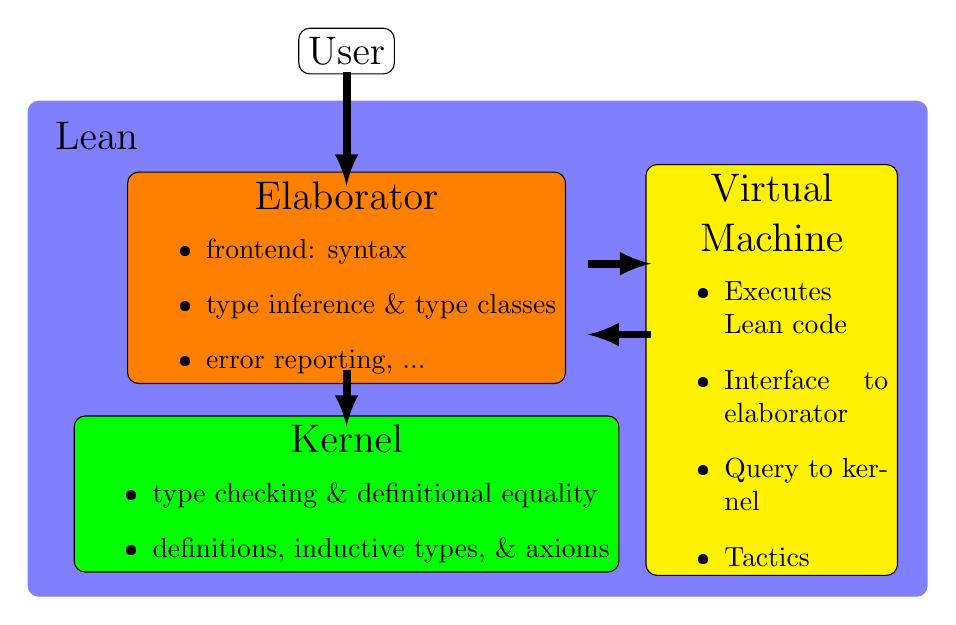
\begin{tikzpicture}[scale=0.9]
    \fill [rounded corners, blue!50!white] (-4.5, -1.7) rectangle (8.2, 5.3) ;
    \node at (-3.5, 4.8) { { \Large Lean } } ;
    \node at (0, 6) [draw, rounded corners] { \Large User };
    \node at (0, 2.8) [draw, rounded corners, fill=orange] {
        \begin{varwidth}{6cm}
        \begin{center} \Large Elaborator \end{center}\vskip -0.5cm
        \begin{itemize}
          \item frontend: syntax
          \item type inference \& type classes
          \item error reporting, ...
        \end{itemize}
      \end{varwidth}
    };
    \node at (0, -0.25) [draw, rounded corners, fill=green] {
        \begin{varwidth}{6.8cm}
        \begin{center} \Large Kernel \end{center}\vskip -0.5cm
        \begin{itemize}
          \item type checking \& definitional equality
          \item definitions, inductive types, \& axioms
        \end{itemize}
      \end{varwidth}
    };
    \node at (6, 1.5) [draw, rounded corners, fill=yellow] {
      \begin{varwidth}{3cm}
      \begin{center} \Large Virtual Machine \end{center}\vskip -0.5cm
      \begin{itemize}
        \item Executes Lean code
        \item Interface to elaborator
        \item Query to kernel
        \item Tactics
      \end{itemize}
    \end{varwidth}
    } ;
    \draw[-latex,line width=1mm] (0, 5.7) -- (0, 4.1);
    \draw[-latex,line width=1mm] (3.4, 3) -- (4.3, 3);
    \draw[-latex,line width=1mm] (4.3, 2) -- (3.4, 2);
    \draw[-latex,line width=1mm] (0, 1.5) -- (0, 0.7);
  \end{tikzpicture}

\end{frame}

\begin{frame}{Object logic vs Meta constants}
  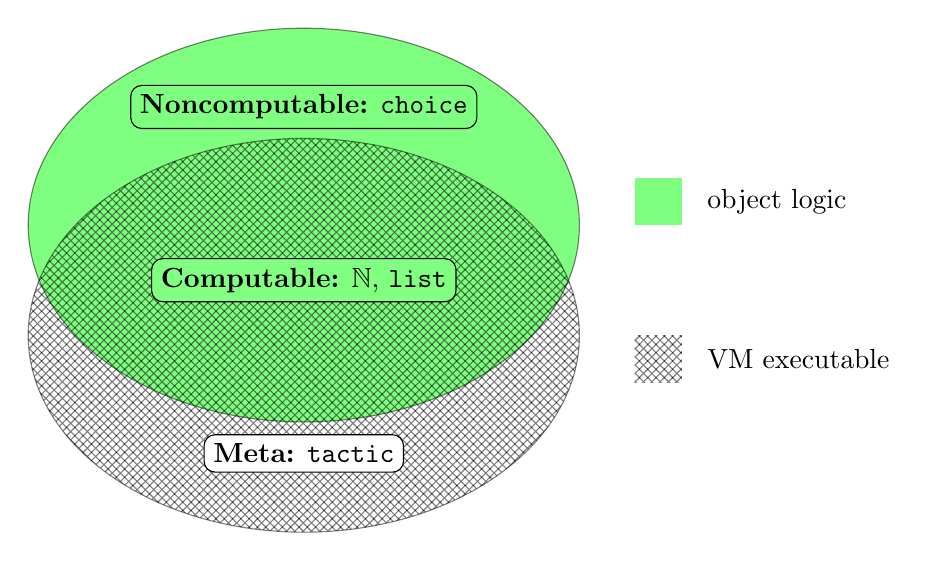
\begin{tikzpicture}
    \draw[opacity = 0.5, fill=green] (0,  0.7) ellipse [x radius=3.5cm, y radius=2.5cm];
    \draw[opacity = 0.5, pattern=crosshatch] (0, -0.7) ellipse [x radius=3.5cm, y radius=2.5cm];
    \node [draw, rounded corners] at (0, 2.2) { \textbf{Noncomputable:} \texttt{choice} };
    \node [fill=green!50!white, rounded corners, draw] at (0, 0) { \textbf{Computable:} $\mathbb{N}$, \texttt{list} };
    \node [fill=white, rounded corners, draw] at (0, -2.2) { \textbf{Meta:} \texttt{tactic} };
    \fill [opacity = 0.5, fill=green] (4.2, 0.7) rectangle (4.8, 1.3);
    \node at (5, 1) [right] {object logic};
    \fill [opacity = 0.5, pattern=crosshatch] (4.2, -0.7) rectangle (4.8, -1.3);
    \node at (5, -1) [right] {VM executable};
  \end{tikzpicture}

\end{frame}

\sect{Lean in \lstinline{meta} Lean}

\begin{frame}[fragile]{How is Lean represented in \lstinline{meta} Lean?}
  \lstinline{meta} types to represent the object logic:
  \begin{description}
    \item[\texttt{name}] hierarchical names \\
      special syntax: \verb$`namespace.name$
    \item[\texttt{level}] represents universe levels
    \item[\texttt{expr}] represents expressions
  \end{description}
\end{frame}

\begin{frame}[fragile]{Expressions in \lstinline{meta} Lean}
\begin{lstlisting}
meta inductive expr (elaborated : bool := tt)
| const    {} : name → list level → expr
| app         : expr → expr → expr
| elet        : name → expr → expr → expr → expr
| sort     {} : level → expr

| lam         :
    name → binder_info → expr → expr → expr
| pi          :
    name → binder_info → expr → expr → expr
| var      {} : nat → expr

| local_const :
    name → name → binder_info → expr → expr
| mvar        : name → name → expr → expr
| macro       : macro_def → list expr → expr
\end{lstlisting}
\end{frame}

\begin{frame}[fragile]{Expressions -- Base}
  \lstinline$const (n : name) (u : list level)$ \\
  \quad $c.\{u_1 \ldots u_n\}$ \\[2ex]
  \lstinline$app (f x : expr)$ \\
  \quad $f~x$ \\[2ex]
  \lstinline$elet (pp : name) (ty t body : expr)$ \\
  \quad $let~pp : ty := t~in~body$ \\[2ex]
  \lstinline$sort (l : level)$ \\
  \quad \lstinline$Sort l$, \lstinline$Type l$, or \lstinline$Prop$ \\[2ex]

  \textbf{Example:} $1 + 0 = 1$ \\
   e.g. \lstinline$@eq.{0} nat (nat.add nat.one nat.zero) nat.one$
\begin{lstlisting}
app (app (app (const `eq [1]) (const `nat []))
  (app (app (const `nat.add []) (const `nat.one [])) (const `nat.zero [])))
  (const `nat.one [])
\end{lstlisting}
\end{frame}

\begin{frame}[fragile]{Expressions - Binders \& Bound Variables}
  \lstinline$lam (pp : name) bi (type : expr) (body : expr)$ \\
  \quad $\lambda (pp : type), body$ \\[2ex]
  \lstinline$pi (pp : name) bi (type : expr) (body : expr)$ \\
  \quad $\Pi (pp : type), body$ \\[2ex]

  How are variables represented in the body of \texttt{lam} and \texttt{pi}?
  \begin{itemize}
    \item \lstinline{var n} is a \emph{bound variable}, referencing a $\lambda$ or $\Pi$
    \item $n$ is the \emph{distance} to the $\lambda$ or $\Pi$ (deBruijn index)
    \item \textbf{Example:} $\lambda (x~y : \mathbb{N}), f~x~y$
\begin{lstlisting}
lam `x default `nat (lam `y default `nat
  (app (app (const `f []) (var 1)) (var 0)))
\end{lstlisting}
    \item \textbf{Advantage:} Expression can be just composed. We don't need to take care of bound variables.
  \end{itemize}
\end{frame}

\begin{frame}[fragile]{Expressions - Local Constants}
  \textbf{Problem:} In the body of a $\lambda$ or $\Pi$ there is only \verb|var n|! \\
  \quad There is no informations about this variables! \\[1ex]

  \textbf{Solution:} Replace \lstinline{var} by \lstinline{local_const}!
  \lstinline{local_const unique pp bi type}
  \begin{description}
    \item[unique] Unique identifier
    \item[pp] User visible (pretty printed) name
    \item[bi] Binder info (implicit, type class instance, \ldots)
    \item[type] The type of the variable
  \end{description}

  \begin{itemize}
    \item Open a $\lambda$ or $\Pi$: replace bound variable by local constant
    \item Close a $\lambda$ or $\Pi$: replace a local constant by bound variable
    \item There are also local universe constants
  \end{itemize}

\end{frame}

\begin{frame}[fragile]{Examples}

\lstinline{∀(α:Type) [monoid α] (a:α), a * 1 = a}

\begin{lstlisting}
pi `α default (sort 1)
  (pi `i inst (app (const `monoid [0]) (var 0))
    (pi `a default (var 1)
      (app (app (app (const `eq [1]) (var 2))
        (app (app (app (app (const `mul [0]) (var 2))
            (var 1)) (var 0))
          (app (app (const `one [0]) (var 2))
            (var 1))))
        (var 0))))
\end{lstlisting}
\end{frame}


\begin{frame}[fragile]{Expressions - Metavariables}

\lstinline$mvar (unique : name) (pp : name) (type : expr)$

\begin{itemize}
\item Metavariables (a.k.a. schematic or existential variables) are holes in expressions.
   \textbf{To be filled in later.}
\item This happens explicitly or by elaboration (using unification)
\item \textbf{Example}:
  Create $x : ?m$, elaborate $x = (0 : \mathbb{N})$, then: $?m := \mathbb{N}$.
\item Is also used to represent goals!
\end{itemize}

\end{frame}

\sect{Tactic framework}

\begin{frame}[fragile]{What is a Tactic?}
  \textbf{Basic idea:}
  \begin{center} \lstinline$tactic := expr → expr$ \end{center}
  \begin{description}
    \item[input] the target as proposition (or type)
    \item[result] is a proof (inhabiting term) of the target
  \end{description}

  \textbf{But this is not enough:}
  \begin{itemize}
    \item Tactics can fail, or return data
    \item Tactics can leave holes in the term, operate on multiple goals
    \item Tactics need access to: local context, attributes, declaration, options,
      meta variables\ldots
    \item We need a tactic state, or a \emph{tactic monad}:
  \end{itemize}
\begin{lstlisting}
tactic α :=
  tactic_state → (α × tactic_state) + error
\end{lstlisting}

\end{frame}

\begin{frame}[fragile]{Tactic State}
  \begin{tikzpicture}
    \fill[blue!50!white] (-5, 0) rectangle (5, 7.7) ;

    \fill[orange] (-1.9, 7.5) rectangle (4.8, 1.5) ;
    \node at (-1.9, 7.5) [below right] {
      \begin{varwidth}{6cm}
        \textbf{Metavariables} \\

\begin{lstlisting}
?m0 : p:Prop ⊢ p → false
?m1 : α:Type, a : α ⊢ a = a
⋯?mn : α:Type, a : α ⊢ …
\end{lstlisting}
  ~\\[2em]
      Assignments: \lstinline$?m2 := rfl, …$
      \end{varwidth}
    } ;

    \fill[orange] (-4.9, 7.5) rectangle (-2.1, 1.5) ;
    \node at (-4.9, 7.5) [below right] {\textbf{Environment}} ;

    \node at (-4.9, 7.1) [below right] {
      \begin{varwidth}{6cm}
        Declarations:
\begin{lstlisting}
true : Prop
nat : Type
zero : nat
\end{lstlisting}
      \dots \\[2em]
      Attributes, \\
      Fresh Names, \\
      etc.

      \end{varwidth}
    };

    \fill[orange] (-4.9, 1.3) rectangle (-2.1, 0.1) ;
    \node at (-4.9, 1.3) [below right] {
      \begin{varwidth}{2.8cm}
        \textbf{Options} \\
        \lstinline$pp.all=tt,..$
      \end{varwidth} } ;

    \fill[orange] (-1.9, 1.3) rectangle (1.8, 0.1) ;
    \node at (-1.9, 1.3) [below right] {
      \begin{varwidth}{3.7cm}
        \textbf{Goals} \\
        \lstinline$[?m0, ..., ?mn]$
      \end{varwidth}
    } ;

    \fill[orange] (2, 1.3) rectangle (4.8 , 0.1) ;
    \node at (2, 1.3) [below right] {
      \begin{varwidth}{2.8cm}
        \textbf{Main Goal} \\
        \lstinline$?m0$
      \end{varwidth}
    } ;

  \end{tikzpicture}
\end{frame}

\end{document}

